\documentclass[9pt,xcolor=table,svgnames]{beamer}
\usepackage{showcode}
% \usetheme{adapt-lab}
\usetheme{customadapt-lab}

% \usepackage{MnSymbol}
\let\Square\undefined
\usepackage{bbding}
\usepackage{pifont}
\usepackage{txfonts}

\usepackage{tabularx}
% \usepackage{bibentry}
\usepackage{booktabs}
\usepackage{tikz}


\title[Toward a Modular Approach for TSs and LSP generation]{Toward a Modular Approach for Type Systems and LSP generation}
% \author{Federico Cristiano Bruzzone}
% \institute{Università degli Studi di Milano \\
%            Facoltà di Scienze e Tecnologie \\
%            Corso di Laurea Magistrale in Informatica \\ [5pt]\vspace{15pt}
%            {\normalsize Advisor: Prof. Walter Cazzola} \\ [1pt]\vspace{5pt}
%            {\normalsize Co-Advisor: Dr. Luca Favalli}}
% \date{July 15\textsuperscript{th} 2024}

\author[Federico Bruzzone]
{\vspace{-10pt}Federico Bruzzone\\\vspace{7pt}{\scriptsize Id. Number: 27427A}}
\institute{\small
	Universit\`a degli Studi di Milano\\
	Computer Science Department\\
	MSc in Computer Science\\\vspace{10pt}
	\begin{tabular}{r l}
        Advisor: & Prof. Walter Cazzola \\
		Co-Advisor: & Dr. Luca Favalli \\
	\end{tabular}
}
\date{\scriptsize{15/07/2024\\\vspace{5pt}LM-18 - Computer science\\Academic Year 2023-2024}}

\tolerance=10
\emergencystretch=\maxdimen
\hyphenpenalty=10000
\hbadness=10000

\begin{document}

\begin{frame}
	\titlepage
\end{frame}

\section{Problem Statement}

\subsection[ ]{Programming Language Implementation}
\begin{frame}{\secname}
    \framesubtitle{\subsecname}
    The implementation of a programming language is a complex task that involves several implementation aspects, such as:

    \begin{tabular}{p{0.5\textwidth} p{0.5\textwidth}}
        \begin{itemize}
            \item Syntax and semantics definition
            \item \alert{Type system definition}
            \item Code generation
        \end{itemize}
        &
        \begin{itemize}
            \item Error handling and recovery
            \item \alert{IDE support}
            \item Documentation
        \end{itemize}
    \end{tabular}

    \pause

    \huge It is usually done in a \alert{monolithic} way, where all the aspects are tightly coupled.

    \pause
    \bigskip

    \normalsize This makes the \alert{maintainability}, \alert{extensibility} and \alert{reusability} of the implementation difficult.
\end{frame}


\subsection[ ]{Type Systems and IDEs Support}
\begin{frame}{\secname}
    \framesubtitle{\subsecname}

    Often some parts of compilation, such as code generation, makes use of {\color{BloodRed} feature-oriented programming} to support different architectures.

    \bigskip
    \pause

    \huge However, the type system and the IDE support are usually implemented using a \alert{top-down} approach.
\end{frame}


% ============================================================================

\section[SPLs]{Software Product Lines}
\subsection[ ]{}

\begin{frame}{\secname}
    \framesubtitle{\subsecname}

    Since 1990s, researchers have been working on the concept of \alert{Software Product Lines} (SPLs) to move towards a more \alert{modular} world.

    \bigskip
    \pause

    \begin{itemize}
        \item SPLs defines a \alert{family} of software products.
        \item SPLs is described by a \alert{Feature Model}.
        \item A Feature Model describes the \alert{variability} of the software.
        \item SPL \alert{variants} are generated by selecting a set of features.
        \item A \alert{feature} (or \alert{artifact}) is a first-class entity in SPLs.
    \end{itemize}
\end{frame}

\subsection[LPLs]{Language Product Lines}
\begin{frame}{\secname}
    \framesubtitle{\subsecname}
    Applying the concept of SPLs to programming languages, we obtain the concept of \alert{Language Product Lines} (LPLs).

    \bigskip
    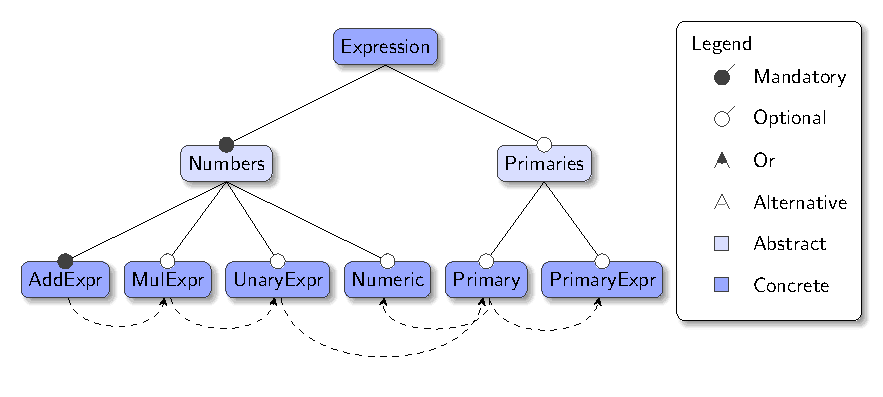
\includegraphics[width=1\textwidth]{figs/feature-model.pdf}

    \pause

    \huge Some achievments:
    \begin{itemize}
        \item \alert{Bottom-up} approach to language implementation
        \item \alert{Reusability} of language artifacts
        \item Multiple \alert{variants} of the same language
        \item \alert{Language Workbenches} come to the rescue
    \end{itemize}
\end{frame}

\subsection[LWs]{Language Workbenches and Neverlang}
\begin{frame}{\secname}
    \framesubtitle{\subsecname}

    \alert{Language Workbenches} (LWs) are tools that allow the development of programming languages, both GPLs and DSLs.

    \scriptsize Some LWs allow the development of LPLs.

    \begin{table}[t]
        \rowcolors{1}{gray!25}{white}
        % \setlength\arrayrulewidth{-1pt}
        \centering
        \resizebox{\textwidth}{!}{%
        \begin{tabular}{ c c c c c c }
            \toprule \textbf{Language Workbench} & \textbf{Modularization Supp.} & \textbf{Precompiled Feature Supp.} & \textbf{Native IDE gen.} & \textbf{LSP Gen.} & \textbf{LSP Mod.} \\
            \midrule
            JustAdd & \LEFTcircle & \Circle & \Circle & \Circle & \Circle \\
            Melange & $\circledwedge$ & \Circle  & 2rd party (EMF) & \ding{80} & \ding{80} \\
            MontiCore & \LEFTcircle & \LEFTcircle & \CIRCLE & \Circle & \Circle \\
            MPS & $\circledwedge$ & \Circle   & \CIRCLE & \ding{79} & \ding{80} \\
            Rascal & \Circle & \Circle & \CIRCLE & \Circle & \Circle \\
            Spoofax & $\circledwedge$  & \LEFTcircle  & \CIRCLE & \ding{79} & \ding{80} \\
            Xtext & \Circle & \LEFTcircle  & \CIRCLE & \CIRCLE & \Circle \\
            Neverlang & $\circledvee$ & \CIRCLE & \Circle & \FiveStarConvex & \FiveStarConvex \\
            \bottomrule
        \end{tabular}
        }
        % \caption{Comparison of language workbenches in terms of modularization, precompiled feature support, native IDE generation, LSP generation, and LSP modularization. The $\CIRCLE$ symbol indicates full support, $\Circle$ no support, $\LEFTcircle$ limited support, $\circledvee$ fine-grained modularization,  $\circledwedge$ coarse-grained modularization, \FiveStarConvex my expected contribution and \ding{79} my expected contribution that can be extended to all LWs that support at least component modularization.}
        \label{tab:lw-comparison}
    \end{table}

    \begin{tabular}{p{0.5\textwidth} p{0.5\textwidth}}
    \begin{itemize}
        \item \CIRCLE Full support
        \item \Circle No support
        \item \LEFTcircle Limited support
        \item $\circledvee$ Fine-grained mod.
    \end{itemize}
    &
    \begin{itemize}
        \item $\circledwedge$ Coarse-grained mod.
        \item \FiveStarConvex My contribution
        \item \ding{80} My contribution extended
   \end{itemize}
   \end{tabular}

    \pause

    \normalsize \alert{Neverlang} is a language workbench, developed by the \alert{ADAPT} lab, that supports the development of LPLs.

\end{frame}

\section[LSP]{Language Server Protocol}

\subsection[The Reductions of Combinations]{The Reduction of Combinations}
\begin{frame}{\secname}
    \framesubtitle{\subsecname}

    In 2016, \alert{Microsoft} in collaboration with \alert{Red Hat} introduced the \alert{Language Server Protocol} (LSP).

    \pause

    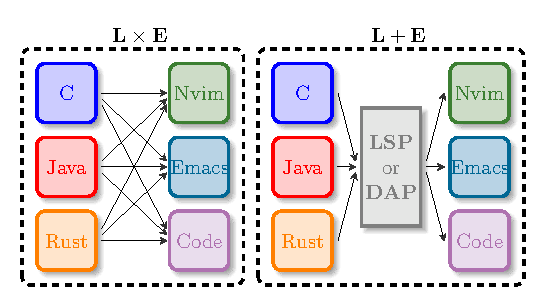
\includegraphics[width=1\textwidth]{figs/lsp-combination.pdf}

    \pause

    \huge Spoiler:
    \normalsize We have reduced the number of combinations from $\mathbf{L} \times \mathbf{E}$ to $\mathbf{N} \times \mathbf{1}$ where $\mathbf{N} \ll \mathbf{L}$.
\end{frame}

\subsection[In a Nutshell]{LSP In a Nutshell}
\begin{frame}{\secname}
    \framesubtitle{\subsecname}

    The \alert{Language Server Protocol} (LSP) is a protocol that allows the communication between a \alert{Language Server} and an \alert{IDE}.

    \pause

    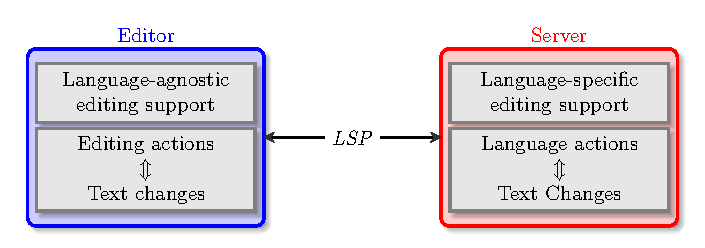
\includegraphics[width=1\textwidth]{figs/lsp-diagram.pdf}

    \begin{tabular}{p{0.5\textwidth} p{0.5\textwidth}}
    Intrinsic properties:
    \begin{itemize}
        \item Language-agnostic
        \item IDE-agnostic
        \item Asynchronous
        \item Text-based
    \end{itemize}
        &
    Features:
    \begin{itemize}
        \item Diagnostics
        \item Hover
        \item Go to definition
        \item Find references
        \item Inlay hints
    \end{itemize}
    \end{tabular}
\end{frame}

% ============================================================================

\section[Scientific Contribution]{Scientific Contribution}

- Type System implementation and a Java Library for Neverlang in order to support the type system for every langauge developed with Neverlang.
- Type System Modularization
- LSP generation for Neverlang languages
- DSL for Type System definition
- Client and Syntax Highlighting generation


\end{document}


